\chapter{METHODOLOGY}
\label{chap:methodology}

This chapter describes the design, implementation, computation, training,
deployment, and evaluation procedures used for the TinyML Smart Plug. The
methodology begins with the system model and firmware flow, then proceeds to
the physical prototype, progressive web application (PWA), TinyML workflow,
sensor calibration, waveform-feature computation, protection logic, and test
procedures. This order follows the flow of the prototype itself: the hardware
measures voltage, current, and temperature; the firmware converts these
measurements into calibrated electrical and thermal variables; the TinyML
pipeline classifies load context and series-arc behavior; and the protection
manager decides whether to warn, log, or disconnect the load.

\section{System Model}
\label{sec:ch3-system-model}

\subsection{Conceptual Framework}
\label{sec:ch3-conceptual-framework}

The prototype was modeled as an input--process--output system. Its inputs were
the mains-voltage sensor, current sensor, thermistor, and wireless connection;
its processing stage was the ESP32-S3 firmware with calibration, thermal
estimation, waveform-feature extraction, TinyML inference, relay control, and
cloud logging; and its outputs were warnings, PWA monitoring, stored event
records, and relay disconnection when a protection condition was latched.

Figure~\ref{fig:ch3-conceptual-framework} summarizes this research model.
\begin{figure}[H]
  \centering
  \begin{tikzpicture}[node distance=0.32in and 0.30in]
    \node[thesis process,text width=1.50in] (inputs) {Inputs\\voltage, current, device temperature, network state};
    \node[thesis process,text width=1.65in,right=of inputs] (processing) {Embedded processing\\calibration, thermal model, waveform features, TinyML inference};
    \node[thesis process,text width=1.50in,right=of processing] (outputs) {Outputs\\warnings, relay action, logs, PWA display/control};
    \node[thesis process,text width=1.45in,below=0.34in of processing] (validation) {Controlled validation\\sensor, overload, socket heating, series arc};
    \node[thesis process,text width=1.45in,below=0.34in of validation] (interpretation) {Interpretation\\complementary protection under tested conditions};
    \draw[thesis arrow] (inputs) -- (processing);
    \draw[thesis arrow] (processing) -- (outputs);
    \draw[thesis arrow] (validation) -- (processing);
    \draw[thesis arrow] (processing) -- (interpretation);
    \draw[thesis arrow] (outputs.south) |- (interpretation.east);
  \end{tikzpicture}
  \caption{Conceptual framework of the TinyML Smart Plug.}
  \label{fig:ch3-conceptual-framework}
\end{figure}

Figure~\ref{fig:ch3-conceptual-framework} shows that the study did not treat
the smart plug as a measurement-only device. The sensing inputs are converted
into protection variables and waveform features, then used to support user
notification, fault logging, and local relay action. This distinction is
important because the prototype was intended as complementary protection, not
as a replacement for branch-circuit breakers, AFCIs, GFCIs, wiring inspection,
or certified protective equipment.

\subsection{System Architecture}
\label{sec:ch3-system-architecture-discussion}

The same behavior can be described as a layered embedded system. The sensing
layer captures voltage, current, and socket temperature; the firmware layer
computes calibrated variables and protection states; the TinyML layer provides
context-aware series-arc inference; and the PWA layer displays live and
historical data using Firebase services [55], [56].

Figure~\ref{fig:ch3-system-architecture} presents the system architecture used
to connect these layers.
\begin{figure}[H]
  \centering
  \begin{tikzpicture}[node distance=0.24in and 0.27in]
    \node[thesis process,text width=1.20in] (sensors) {Sensors\\voltage, current, temperature};
    \node[thesis process,text width=1.55in,right=of sensors] (esp) {TinyML Smart Plug\\ESP32-S3 local protection};
    \node[thesis process,text width=1.28in,right=of esp] (relay) {Relay and\\protected outlet};
    \node[thesis process,text width=1.28in,above=0.30in of relay] (local) {OLED, buzzer,\\local indicators};
    \node[thesis process,text width=1.38in,below=0.32in of esp] (firebase) {Firebase\\Realtime Database};
    \node[thesis process,text width=1.42in,right=of firebase] (pwa) {PWA\\visualization, logs, basic control};
    \draw[thesis arrow] (sensors) -- (esp);
    \draw[thesis arrow] (esp) -- node[above,font=\scriptsize]{local trip} (relay);
    \draw[thesis arrow] (esp) -- (local);
    \draw[thesis arrow] (esp) -- node[left,font=\scriptsize]{telemetry} (firebase);
    \draw[thesis arrow] (firebase) -- node[above,font=\scriptsize]{live data} (pwa);
    \draw[thesis arrow] (pwa.south west) -- node[below,font=\scriptsize]{clear/relay commands} (firebase.south east);
    \draw[thesis arrow] (firebase.north) -- node[left,font=\scriptsize]{control fields} (esp.south);
  \end{tikzpicture}
  \caption{System architecture of the TinyML Smart Plug.}
  \label{fig:ch3-system-architecture}
\end{figure}

Figure~\ref{fig:ch3-system-architecture} places the ESP32-S3 at the center of
the design. The microcontroller receives conditioned analog signals, runs the
protection and TinyML routines locally, drives the relay and indicators, and
uploads selected telemetry. Firebase and the PWA also carry basic remote
control fields, such as fault clearing and relay-control commands, but these
commands do not replace the local protection logic. Keeping the protection
decision on the
microcontroller prevents the relay action from depending on internet
availability, while the cloud and PWA remain useful for visualization,
logging, labeling, review, and operator interaction.

\subsection{Input, Processing, and Output Summary}
\label{sec:ch3-system-ipo}

The design variables used by the system are summarized in
Table~\ref{tab:ch3-system-variables}. The table separates direct measurements
from computed variables so that later equations can be traced to the firmware
implementation.
\begin{table}[H]
  \centering
  \caption{Main firmware variables used by the prototype}
  \label{tab:ch3-system-variables}
  \begin{tabular}{p{0.25\textwidth}p{0.28\textwidth}p{0.35\textwidth}}
    \toprule
    \textbf{Variable group} & \textbf{Source} & \textbf{Application} \\
    \midrule
    RMS voltage & ZMPT101B channel and voltage calibration & Voltage monitoring, mains-present logic, undervoltage and overvoltage protection \\
    RMS current & ACS37035 channel, MCP3204 ADC, anti-aliasing filter, and current calibration & Load monitoring, overload protection, thermal load term, and arc-feature extraction \\
    Device temperature measurement & 10k$\Omega$ thermistor and divider computation & Baseline thermal measurement for socket-temperature estimation \\
    Waveform features & Current samples processed by the arc-detection module & Context classification and Random Forest arc inference \\
    Protection state & Protection manager and relay driver & Warning, latching, relay disconnection, and event logging \\
    \bottomrule
  \end{tabular}
\end{table}

Table~\ref{tab:ch3-system-variables} shows that current is used by several
subsystems: it supports ordinary overload detection, thermal compensation, and
the TinyML feature vector. Therefore, the current channel was treated as a
shared measurement path whose calibration and sampling behavior must remain
consistent across protection functions.

\section{Program and Firmware Flow}
\label{sec:ch3-program-flow}

\subsection{Initialization and Sampling}
\label{sec:ch3-initialization-sampling}

The firmware follows a repeated acquisition, computation, inference, and
protection cycle. On startup, the ESP32-S3 initializes the sensors, relay
driver, OLED display, buzzer, Wi-Fi, Firebase interface, and local protection
state. In the main loop, it samples the voltage, thermistor, and current
waveform, applies calibration and filtering, computes thermal and waveform
features, updates the context classifier, evaluates the arc classifier, and
passes the resulting variables to the protection manager.

Figure~\ref{fig:ch3-program-flow} shows the operating sequence implemented by
the firmware.
\begin{figure}[H]
  \centering
  
\includegraphics[width=0.96\textwidth]{ch3/figure_3.3.png}
  \caption{Program flowchart of the TinyML Smart Plug firmware.}
  \label{fig:ch3-program-flow}
\end{figure}

\subsection{Protection-State Evaluation}
\label{sec:ch3-protection-state-evaluation}

Figure~\ref{fig:ch3-program-flow} shows that a relay trip can be caused by a
sustained overload, an estimated socket over-temperature, or an arc-fault
classification. The overload path issues a warning above 10.0A, but relay
disconnection is based on persistence above 14.5A. This persistence is
implemented as a score that increases every 10s while the
condition remains active and trips when the score reaches 6, equivalent to
approximately 60s of sustained overload. This makes the overload behavior
closer to inverse-time protection logic than to an instantaneous cutoff [22].

The firmware also latches fault states. After relay disconnection, the event is
recorded locally and uploaded when the network is available. The plug remains
in the fault state until the user clears the fault through the device or
application workflow. This prevents a hazardous load from being automatically
re-energized after a transient communication or reset event.

\subsection{Timing Constants}
\label{sec:ch3-timing-constants}

The sampling and timing constants used by the firmware are listed in
Table~\ref{tab:ch3-firmware-constants}. These values were taken from the
firmware configuration and the current-sensing implementation.
\begin{table}[H]
  \centering
  \caption{Selected firmware timing and sampling constants}
  \label{tab:ch3-firmware-constants}
  \begin{tabular}{p{0.38\textwidth}p{0.22\textwidth}p{0.30\textwidth}}
    \toprule
    \textbf{Constant} & \textbf{Value} & \textbf{Role} \\
    \midrule
    Target current sampling rate & 27,000Hz & Current waveform acquisition for feature extraction \\
    Arc runtime frame length & 512 samples & FFT and time-domain feature window \\
    Arc runtime hop length & 256 samples & Overlap between consecutive feature frames \\
    Feature emission cadence & Every 3 hops & Approximate 35.16Hz feature output rate \\
    MCP3204 SPI clock & 1.2MHz & 12-bit current ADC transfer clock \\
    Voltage sampling interval & 250 $\mu$s & Firmware voltage-window acquisition interval \\
    \bottomrule
  \end{tabular}
\end{table}

Table~\ref{tab:ch3-firmware-constants} explains why the current path is
handled separately from slow telemetry. Arc-fault detection requires waveform
frames with millisecond-scale timing, while Firebase updates and PWA displays
operate at a slower human-monitoring cadence.

\section{PWA and Monitoring System}
\label{sec:ch3-pwa-monitoring}

The monitoring system was implemented as a PWA connected to Firebase. The PWA
was not placed in the protection path; the ESP32-S3 still made relay decisions
locally. The PWA instead provided live measurements, protection status, event
history, CSV download, labeling support, and review of waveform-derived
features. This separation allowed the prototype to remain protective during
network loss while still supporting data collection and analysis.

Figure~\ref{fig:ch3-pwa-block} shows the PWA data path.
\begin{figure}[H]
  \centering
  
\includegraphics[width=0.82\textwidth]{ch3/figure_3.12.png}
  \caption{PWA block diagram and Firebase data path.}
  \label{fig:ch3-pwa-block}
\end{figure}

Figure~\ref{fig:ch3-pwa-block} shows that the firmware publishes selected
telemetry to Firebase, while the browser-based PWA subscribes to the same data
for display and logging. This arrangement matches the PWA role described in
Firebase documentation: the web client improves access and installation
behavior, but the embedded device remains responsible for field decisions
[55], [56].

The live dashboard used during testing is shown in
Figure~\ref{fig:ch3-pwa-dashboard}.
\begin{figure}[H]
  \centering
  
\includegraphics[width=0.92\textwidth]{ch3/figure_3.13.png}
  \caption{Actual PWA live dashboard.}
  \label{fig:ch3-pwa-dashboard}
\end{figure}

Figure~\ref{fig:ch3-pwa-dashboard} displays voltage, current, direct NTC
temperature, estimated socket temperature, THD, spectral features, protection
state, and relay state. The dashboard intentionally distinguishes direct NTC
temperature from estimated socket temperature because the relay-facing thermal
decision uses the compensated estimate, not the raw thermistor reading alone.

The event-history page is shown in Figure~\ref{fig:ch3-pwa-history}.
\begin{figure}[H]
  \centering
  
\includegraphics[width=0.92\textwidth]{ch3/figure_3.14.png}
  \caption{Actual PWA history-log view.}
  \label{fig:ch3-pwa-history}
\end{figure}

Figure~\ref{fig:ch3-pwa-history} documents the stored-event interface used to
review warnings, trips, and data records after tests. The history function was
also useful for checking whether the firmware sequence matched the expected
warning, persistence, and latching behavior during overload, heating, and
arc-fault trials.

\section{Telemetry Fields}
\label{sec:ch3-telemetry-fields}

The PWA displayed only a selected subset of firmware variables. The most
important telemetry fields are listed in Table~\ref{tab:ch3-telemetry}.
\begin{table}[H]
  \centering
  \caption{Selected telemetry fields shown in the PWA}
  \label{tab:ch3-telemetry}
  \begin{tabular}{p{0.30\textwidth}p{0.25\textwidth}p{0.35\textwidth}}
    \toprule
    Field & Firmware source & Interpretation \\
    \midrule
    Voltage and current & Calibrated sensor routines & Electrical state of the connected load \\
    NTC temperature & Thermistor routine & External temperature at the sensor position \\
    Estimated socket temperature & Thermal estimator & Protection-facing estimate of socket temperature \\
    Arc probability and class & Random Forest inference & TinyML arc-fault decision support \\
    Context family and confidence & Context prototype model & Load-family estimate used by arc-threshold selection \\
    Relay and fault state & Protection manager & Whether the load is energized or latched off \\
    \bottomrule
  \end{tabular}
\end{table}

Table~\ref{tab:ch3-telemetry} shows that the PWA was both an operator display
and a research instrument. During data collection, these fields allowed the
researchers to compare raw measurements, computed estimates, and protection
outputs in the same session record.

\section{Physical Setup and Hardware Implementation}
\label{sec:ch3-physical-setup}

\subsection{Sensing Subsystems and Hardware Blocks}
\label{sec:ch3-sensing-subsystems}

The physical implementation combined a line-side plug, protected outlet,
solid-state relay module, ESP32-S3 controller, voltage sensor, current sensor,
NTC thermistor, anti-aliasing circuit, backup supply, OLED display, buzzer,
and enclosure. The hardware was organized so that mains conductors, sensing
circuits, low-voltage logic, and user-interface wiring could be traced
separately during testing.

Figure~\ref{fig:ch3-block-diagram} gives the hardware block-level view before
the detailed schematic is introduced.
\begin{figure}[H]
  \centering
  
\includegraphics[width=0.98\textwidth]{ch3/figure_3.4.png}
  \caption{Block diagram of the prototype hardware.}
  \label{fig:ch3-block-diagram}
\end{figure}

Figure~\ref{fig:ch3-block-diagram} shows that the relay is positioned as the
final protective actuator, while the voltage, current, and temperature sensors
serve as inputs to the ESP32-S3. This placement allows the firmware to remove
power from the protected outlet after a protection condition is confirmed.

\subsection{Full Schematic Discussion}
\label{sec:ch3-full-schematic-discussion}

The full circuit schematic is shown in Figure~\ref{fig:ch3-full-schematic}.
\clearpage
\begin{figure}[p]
  \centering
  
\includegraphics[angle=90,width=0.96\textheight,height=0.96\textwidth,keepaspectratio,trim=0.20in 0.55in 0.20in 0.25in,clip]{ch3/full_schematic.pdf}
  \caption{Full schematic of the TinyML Smart Plug prototype.}
  \label{fig:ch3-full-schematic}
\end{figure}
\clearpage

Figure~\ref{fig:ch3-full-schematic} shows the prototype as several functional
sections rather than as one undifferentiated circuit. The AC input enters the
line-side plug and passes toward the protected outlet through the relay or
load-isolation path, so the relay is the firmware-controlled actuator that
disconnects the load after a latched trip. The voltage-sensing path is taken
from the AC input through the ZMPT101B module and is used only as a monitored
signal for RMS voltage and mains-present logic. The current-sensing path
places the ACS37035 in the load path, routes the conditioned output through
the anti-aliasing and signal-conditioning stage, and digitizes the result with
the MCP3204 ADC for both RMS current and waveform-feature extraction.

The ESP32-S3 section receives the ADC, voltage, and thermistor signals, then
drives the relay-latching circuit, OLED, buzzer, and local indicators. Wi-Fi
communication is handled by the ESP32-S3 and links the local firmware to the
Firebase/PWA monitoring path; the relay decision itself remains local. The
power-supply section separates the low-voltage control electronics from the AC
input through the module supply and local regulators, while signal returns for
the low-voltage circuits are kept within the control side of the prototype.
The schematic supports bench validation of the prototype architecture, but it
does not by itself certify creepage, clearance, enclosure safety, regulatory
compliance, or suitability as a replacement for listed protective devices.
The board-layout views that support this schematic are provided in
Appendix~\ref{app:b}.

\subsection{Signal Conditioning and Enclosure Implementation}
\label{sec:ch3-signal-conditioning-enclosure}

The anti-aliasing circuit and its frequency response are shown in
Figures~\ref{fig:ch3-aaf-circuit} and~\ref{fig:ch3-aaf-bode}.
\begin{figure}[H]
  \centering
  
\includegraphics[width=0.70\textwidth]{ch3/figure_3.6.png}
  \caption{Second-order multiple-feedback low-pass anti-aliasing circuit.}
  \label{fig:ch3-aaf-circuit}
\end{figure}

\begin{figure}[H]
  \centering
  
\includegraphics[width=0.70\textwidth]{ch3/figure_3.7.png}
  \caption{Bode response of the anti-aliasing filter.}
  \label{fig:ch3-aaf-bode}
\end{figure}

Figure~\ref{fig:ch3-aaf-circuit} shows the analog low-pass filter placed
between the current sensor and the ADC. Figure~\ref{fig:ch3-aaf-bode} verifies
that the filter attenuates higher-frequency content before sampling. The
implemented firmware also applies a digital soft anti-aliasing filter in the
current-feature path, so the analog and digital filters work together rather
than as isolated design elements [57].

The internal arrangement was first modeled before assembly. Figure~\ref{fig:ch3-model-no-case}
shows the prototype layout without the case.
\begin{figure}[H]
  \centering
  
\includegraphics[width=0.85\textwidth]{ch3/figure_3.8.png}
  \caption{Three-dimensional model of the prototype without the case.}
  \label{fig:ch3-model-no-case}
\end{figure}

Figure~\ref{fig:ch3-model-no-case} was used to check the relative placement of
the PCB, outlet, relay, fan, and front-panel controls before final enclosure
assembly. This reduced the chance that the enclosure would interfere with
airflow, wiring, or user access.

The corresponding assembled device without the outer case is shown in
Figure~\ref{fig:ch3-actual-no-case}.
\begin{figure}[H]
  \centering
  
\includegraphics[width=0.85\textwidth]{ch3/figure_3.9.png}
  \caption{Actual prototype assembly without the case.}
  \label{fig:ch3-actual-no-case}
\end{figure}

Figure~\ref{fig:ch3-actual-no-case} confirms that the physical wiring followed
the planned internal organization. The exposed view was used during bench
testing to probe the sensing, supply, relay, and communication subsystems.

The enclosure model is shown in Figure~\ref{fig:ch3-model-with-case}.
\begin{figure}[H]
  \centering
  
\includegraphics[width=0.85\textwidth]{ch3/figure_3.10.png}
  \caption{Three-dimensional model of the prototype with the case.}
  \label{fig:ch3-model-with-case}
\end{figure}

Figure~\ref{fig:ch3-model-with-case} shows the intended user-facing
arrangement: outlet access, front controls, ventilation, and rear plug
connection. The enclosure therefore served both a mechanical and an
operator-interface purpose.

The completed enclosed prototype is shown in Figure~\ref{fig:ch3-actual-with-case}.
\begin{figure}[H]
  \centering
  
\includegraphics[width=0.85\textwidth]{ch3/figure_3.11.png}
  \caption{Actual prototype with the case installed.}
  \label{fig:ch3-actual-with-case}
\end{figure}

Figure~\ref{fig:ch3-actual-with-case} shows the plug side and outlet side of
the completed device. This view documents the final physical form used for the
overload, socket-heating, and series arc-fault tests described later in this
chapter.

The major hardware elements are summarized in Table~\ref{tab:ch3-hardware}.
\begin{table}[H]
  \centering
  \caption{Major hardware elements of the prototype}
  \label{tab:ch3-hardware}
  \begin{tabular}{p{0.30\textwidth}p{0.25\textwidth}p{0.35\textwidth}}
    \toprule
    \textbf{Subsystem} & \textbf{Components} & \textbf{Application} \\
    \midrule
    Microcontroller & ESP32-S3 & Local computation, Wi-Fi communication, TinyML inference, relay control \\
    Voltage sensing & ZMPT101B module & RMS voltage measurement and voltage protection input \\
    Current sensing & ACS37035 with MCP3204 ADC & RMS current measurement and waveform-feature source \\
    Temperature sensing & 10k$\Omega$ thermistor & Device temperature measurement for thermal estimation \\
    Protection actuator & Solid-state relay module & Load disconnection after latched protection condition \\
    User interface & OLED, buzzer, LEDs, PWA & Local and remote warning and monitoring \\
    \bottomrule
  \end{tabular}
\end{table}

Table~\ref{tab:ch3-hardware} shows that the prototype combines conventional
sensing and switching hardware with local embedded inference. The hardware
alone does not determine the protection behavior; the firmware computations in
the following sections define how the raw signals are interpreted.

\section{TinyML Development and Deployment Workflow}
\label{sec:ch3-tinyml-workflow}

The TinyML workflow used logged current-waveform features to train two embedded
models: a load-context model and a series arc-fault model. The context model
estimated the appliance family during the early stable portion of a load run.
Its load-family output was then used as an input to the arc model, where it was
encoded as context fields. The arc model combined selected arc-sensitive
features with that context output to classify whether a frame was consistent
with a series arc fault.
Random Forest classification was selected because it can model nonlinear
feature interactions while remaining exportable as a compact tree ensemble for
microcontroller execution [68], [69].
\begin{figure}[H]
  \centering
  \resizebox{0.75\textwidth}{!}{%
  \begin{tikzpicture}[node distance=0.30in and 0.42in]
    \node[thesis process,text width=1.38in] (bench) {Bench tests\\normal, start, arc};
    \node[thesis process,text width=1.38in,right=of bench] (log) {Firmware CSV\\feature logs};
    \node[thesis process,text width=1.38in,right=of log] (label) {Manual review\\labels and notes};

    \node[thesis process,text width=1.38in,below=0.36in of label] (prepare) {Python data\\cleaning and splits};
    \node[thesis process,text width=1.38in,left=of prepare] (context) {Context model\\training};
    \node[thesis process,text width=1.38in,left=of context] (arc) {Random Forest\\arc training};

    \node[thesis process,text width=1.38in,below=0.36in of arc] (metrics) {Metrics\\confusion reports};
    \node[thesis process,text width=1.38in,right=of metrics] (export) {Exported C\\model headers};
    \node[thesis process,text width=1.38in,right=of export] (deploy) {Firmware\\integration and tests};

    \draw[thesis arrow] (bench) -- (log);
    \draw[thesis arrow] (log) -- (label);
    \draw[thesis arrow] (label) -- (prepare);
    \draw[thesis arrow] (prepare) -- (context);
    \draw[thesis arrow] (context) -- (arc);
    \draw[thesis arrow] (arc) -- (metrics);
    \draw[thesis arrow] (metrics) -- (export);
    \draw[thesis arrow] (export) -- (deploy);
  \end{tikzpicture}}
  \caption{Data logging, labeling, and TinyML deployment workflow.}
  \label{fig:ch3-data-labeling-deploy}
\end{figure}

\textit{Figure~\ref{fig:ch3-data-labeling-deploy}} shows that the training workflow was
not performed directly on the microcontroller. The firmware generated CSV
records from bench tests, the records were reviewed and labeled, and Python
scripts then cleaned the rows, formed training and test splits, trained the
context and arc models, computed confusion reports, and exported C headers.
The final embedded test was therefore a deployment check of the exported
headers inside the firmware, not a new training step on the ESP32-S3. This
follows the usual TinyML pattern of offline training followed by
resource-constrained on-device execution [43], [73].
\begin{figure}[H]
  \centering
  \resizebox{0.56\textwidth}{!}{%
  \begin{tikzpicture}[node distance=0.24in and 0.60in]
    \node[thesis process,text width=1.75in] (frame) {Current waveform\\512-sample frame};
    \node[thesis process,text width=1.75in,below=of frame] (features) {Computed/logged\\20 waveform fields};
    \node[thesis process,text width=1.75in,below=of features] (context) {Context model\\6 selected inputs};
    \node[thesis process,text width=1.75in,right=of context] (family) {Load-family\\code and confidence};
    \node[thesis process,text width=1.75in,below=of context] (arcvec) {Arc input vector\\6 waveform + 7 context};
    \node[thesis process,text width=1.75in,below=of arcvec] (rf) {Random Forest\\arc probability};
    \node[thesis process,text width=1.75in,below=of rf] (persist) {Persistence\\counter and latch};
    \node[thesis process,text width=1.75in,below=of persist] (relay) {Local relay,\\alerts, and logs};

    \node[thesis process,text width=1.75in,right=of features] (pwa) {Firebase/PWA\\10 live feature cards\\logging and control};

    \draw[thesis arrow] (frame) -- (features);
    \draw[thesis arrow] (features) -- (context);
    \draw[thesis arrow] (context) -- (arcvec);
    \draw[thesis arrow] (context) -- (family);
    \draw[thesis arrow] (family) |- (arcvec);
    \draw[thesis arrow] (arcvec) -- (rf);
    \draw[thesis arrow] (rf) -- (persist);
    \draw[thesis arrow] (persist) -- (relay);
    \draw[thesis arrow] (features) -- (pwa);
  \end{tikzpicture}}
  \caption{TinyML processing sequence from feature logging to embedded inference.}
  \label{fig:ch3-tinyml-sequence}
\end{figure}

\textit{Figure~\ref{fig:ch3-tinyml-sequence}} shows that the firmware computes feature
fields first, then updates context, then evaluates the arc classifier. This
order is important because the deployed arc header includes both waveform
features and context fields. The load-family result is therefore not only a
display label; when confidence is sufficient, it becomes part of the input
context supplied to the arc model. The flowchart also separates three feature
sets: the candidate fields computed and logged by the firmware, the six base
waveform features selected for the deployed arc model, and the 10 live
feature cards shown by the PWA. A broader 14-feature order remains in the PWA
metadata and session viewer for historical review and CSV inspection.

Arc labels were assigned from logged waveform sessions. The labeling interface
is shown in \textit{Figure~\ref{fig:ch3-arc-labeling}}.
\begin{figure}[H]
  \centering
  
\includegraphics[width=0.99\textwidth]{ch3/figure_3.28.png}
  \caption{Arc labeling using logged waveform data.}
  \label{fig:ch3-arc-labeling}
\end{figure}

\textit{Figure~\ref{fig:ch3-arc-labeling}} shows the interface used to mark arc
events from the logged waveform sessions. The labels were based on the
observed test action and on the expected behavior of series arcs during
contact separation and restriking. Because the marking was done manually
after the test, the selected points are not exact arc-onset locations, but
time-aligned approximations near the RMS waveform changes associated with
the disconnection and recontact events.

To account for this labeling uncertainty, the training set did not treat
only the marked row as the arc event. Neighboring rows around each arc marker
were also given soft arc weights so that brief timing delays in the manual
marking would not force nearby arc-related frames to be learned as normal
behavior. This is presented in \textit{Appendix F} and is also shown in 
\textit{Figure~\ref{fig:ch3-python-trainer}}.
\begin{figure}[H]
  \centering
  
\includegraphics[width=0.99\textwidth]{ch3/figure_3.29.png}
  \caption{Local Python TinyML trainer.}
  \label{fig:ch3-python-trainer}
\end{figure}

\textit{Figure~\ref{fig:ch3-python-trainer}} documents the offline training environment
used to prepare the exported embedded model files. The workflow used separate
data preparation, context-model training, Random Forest training, shared
TinyML utility, and generation-path routines as the source of truth for
feature selection, data splits, hyperparameter search, metric computation,
and embedded export. The dataset-preparation, training-report, and exported
embedded-model summaries are provided in
\textit{Appendix~\ref{app:f-tinyml-training-summary}}.

\subsection{Context Model}
\label{sec:ch3-context-model}

The load context model is a centroid classifier, not a
Random Forest. The context model defines six input features:
$\Delta I_{\mathrm{rms}}$, half-cycle asymmetry, midband residual
ratio, current THD, mid/high-frequency spectral flux, and high-frequency
energy delta. These features were used because they describe the waveform
behavior of the connected load rather than a single fault event.
For example, different load families may exhibit different harmonic content,
asymmetry, and current-change patterns even during normal operation.

In this study, the context model was used to provide load-family information
to the arc classifier, but its experimental coverage was still limited by the
available tested loads. As stated in the limitations of the study, the actual
collected and tested load signatures were limited to resistive loads,
inductive loads, and brushed motor loads.

During runtime, the firmware averages usable feature frames over the
acquisition interval, standardizes each averaged feature, computes the
squared Euclidean distance to each family centroid, and applies a softmax to
the negative distances:
\begin{equation}
  p_c =
  \frac{\exp(-d_c^2)}
       {\sum_{j=1}^{C}\exp(-d_j^2)},
  \qquad
  d_c^2 = \sum_{i=1}^{m}
  \left(\frac{x_i-\mu_i}{\sigma_i}-q_{c,i}\right)^2 .
  \label{eq:context-prototype}
\end{equation}
In \eqref{eq:context-prototype}, $p_c$ is the context confidence for family
$c$, $x_i$ is the averaged runtime feature, $\mu_i$ and $\sigma_i$ are the
training-set mean and standard deviation exported in the header, $q_{c,i}$ is
the standardized centroid coordinate for family $c$, $m=6$ is the context
input dimension, and $C=6$ is the number of load families. A family is accepted
only when the best confidence is at least 0.45; otherwise, the context remains
unknown. This threshold prevents weak or ambiguous feature patterns from being
forced into a load family.

The context acquisition constants in the firmware require a load to remain
active before the context is latched. A provisional context may be used after
the minimum acquisition period, and the final context is latched after the
configured 5s acquisition window when confidence is sufficient. This prevents
brief startup artifacts from immediately forcing a load family into the arc
classifier. Once the context is latched, it remains stable for the continuous
load run, so the arc model receives a consistent family condition during
normal monitoring. The context is returned to unknown only after the load has
been inactive long enough to indicate that the previous operating condition
has ended.

\subsection{Arc Model}
\label{sec:ch3-arc-model}

The deployed series-arc classifier is the Random Forest used by the embedded
arc model. The deployed Random Forest arc model defines 13 inputs: six
base waveform features, six one-hot context-family fields, and one context
confidence field. The base features are maximum low-current run, zero-dwell
ratio, low-current ratio, absolute RMS-current z-score relative to baseline,
midband residual ratio, and mid/high-frequency spectral flux. These were
selected because series arcs can produce current interruption, restrike spikes,
cycle-to-cycle waveform disturbance, and broadband spectral changes [34],
[35], [50], [53]. Since the reviewed literature also shows that series arcs
are load-dependent and difficult to detect using current magnitude alone, the
arc decision was implemented as a multi-feature classifier rather than as a
single-threshold current decision [33], [34], [36].

The first three base features describe current dropouts and low-current
intervals that may occur when a contact separates. The RMS-current z-score
compares the present current behavior with the recent baseline, allowing the
model to detect abrupt deviations from the expected operating level. The
midband residual ratio and mid/high-frequency spectral flux describe waveform
disturbance and spectral changes that may occur during restriking. Together,
these features allow the model to observe both the time-domain interruption
and the frequency-domain disturbance caused by a possible arc event. This
follows the reviewed arc-fault studies, where zero-current behavior,
current-fluctuation features, high-frequency noise, and spectral changes were
used as indicators of series arcing [34]-[39], [49]-[53].

The context-family inputs allow the arc classifier to interpret the same
waveform features differently depending on the connected load type. This is
important because some normal loads, such as motors or phase-controlled
devices, can naturally produce distorted or non-sinusoidal current waveforms.
The context confidence is included so that the model can also account for how
reliable the assigned load family is. When the context is unknown or weak, the
arc decision is treated more conservatively to reduce false operation during
unstable startup or ambiguous load behavior. This follows the reviewed NILM
and load-family literature, where load signatures were shown to affect how
waveform features should be interpreted [8], [40]-[42].

Random Forest was used because the reviewed TinyML literature supports compact
feature-based models that can be deployed on constrained embedded hardware
when the feature space and runtime are carefully designed [32], [43]. In this
study, the Random Forest therefore serves as the embedded decision layer that
combines the selected arc-related features and the estimated load context.
\begin{table}[H]
  \centering
  \caption{Deployed Random Forest arc-model settings}
  \label{tab:ch3-arc-model-export}
  \begin{tabular}{p{0.36\textwidth}p{0.22\textwidth}p{0.32\textwidth}}
    \toprule
    \textbf{Item} & \textbf{Deployed value} & \textbf{Source or role} \\
    \midrule
    Model type & Random Forest & Exported tree ensemble from the local training workflow \\
    Input dimension & 13 & Six waveform features plus seven context fields \\
    Base feature count & 6 & Arc-sensitive features used before context fields \\
    Default arc threshold & 0.4800 & Probability threshold for supported context families \\
    Context confidence minimum & 0.4500 & Minimum accepted context confidence \\
    Unknown-context threshold & 0.7800 & More conservative threshold when context is unknown \\
    Unknown minimum feature votes & 3 & Additional runtime safeguard for unknown-context decisions \\
    \bottomrule
  \end{tabular}
\end{table}

\textit{Table~\ref{tab:ch3-arc-model-export}} shows that the deployed inference was
context-aware. The model used lower thresholds for selected known families and
a higher threshold for unknown contexts, reducing nuisance trips when the load
family could not be established confidently. The firmware then passed the arc
classification to the protection manager, where a leaky counter required
persistence before relay disconnection.

\subsection{Feature Selection for the Deployed Arc Model}
\label{sec:ch3-arc-feature-selection}

The exported firmware header is the source of truth for the deployed feature
selection. It defines 13 arc-model inputs: six waveform features and seven
context fields. Therefore, this paper treats the context one-hot fields
and context confidence as model inputs, but not as additional waveform
features. The selected waveform features are maximum low-current run,
zero-dwell ratio, low-current ratio, absolute RMS-current z-score relative to
baseline, midband residual ratio, and mid/high-frequency spectral flux. The
full computed/logged feature contract is given in
\textit{Section~\ref{sec:ch3-waveform-features}}.

\subsection{Training Split and Model Evaluation}
\label{sec:ch3-training-split}

The Random Forest report, as documented in \textit{Appendix F}, shows that the final arc dataset was split into
35,512 training rows, 9,434 validation rows, and 10,268 test rows. The final
training report used 5 cross-validation splits during search and reported the
held-out test metrics after model selection. The best exported hyperparameters
were 160 trees, maximum tree depth of 16, minimum leaf size of 4, minimum split
size of 12, maximum feature fraction of 0.35, bootstrap sampling enabled, and
entropy criterion. Train/test splitting, cross-validation, and confusion-matrix
metrics are standard model-evaluation practices for supervised classification
[69], [74].

The held-out test-set confusion matrix in the exported report contained 10,173
true negatives, 5 false positives, 25 false negatives, and 65 true positives.
The corresponding frame-level accuracy, precision, recall, and F1-score were
99.7078\%, 92.8571\%, 72.2222\%, and 81.25\%, respectively. Event-level
evaluation was also reported because arc faults occur in grouped episodes
rather than as isolated independent frames; the event-level recall was 84.0\%,
with one false-alarm event in the test sessions.

\section{Sensor Calibration and Computations}
\label{sec:ch3-sensor-calibration}

Sensor calibration converted raw sensor-derived values into engineering units
used by the protection routines. Polynomial calibration was used for the
voltage and current channels because the measured sensor outputs were not
perfectly proportional to the reference instruments over the tested range.
Ordinary least-squares regression estimates coefficients by minimizing the sum
of squared residuals between the measured and fitted values [71]. The
calibration coefficients below were verified from the firmware configuration.
The raw calibration records are retained in Appendix~\ref{app:a},
specifically Tables~\ref{tab:app-a-voltage-calibration},
\ref{tab:app-a-current-calibration}, and
\ref{tab:app-a-temperature-calibration}.

\subsection{Voltage Calibration}
\label{sec:ch3-voltage-calibration}

The voltage calibration setup is shown in
Figure~\ref{fig:ch3-voltage-cal-setup}.
\begin{figure}[H]
  \centering
  
\includegraphics[width=0.90\textwidth]{ch3/figure_3.17.png}
  \caption{Data-collection setup for voltage calibration.}
  \label{fig:ch3-voltage-cal-setup}
\end{figure}

Figure~\ref{fig:ch3-voltage-cal-setup} shows the prototype voltage channel
being compared with reference multimeters while the applied voltage was varied.
The calibration target was the reference RMS voltage, not the uncorrected
sensor output.

The fitted voltage regression is shown in
Figure~\ref{fig:ch3-voltage-regression}.
\begin{figure}[H]
  \centering
  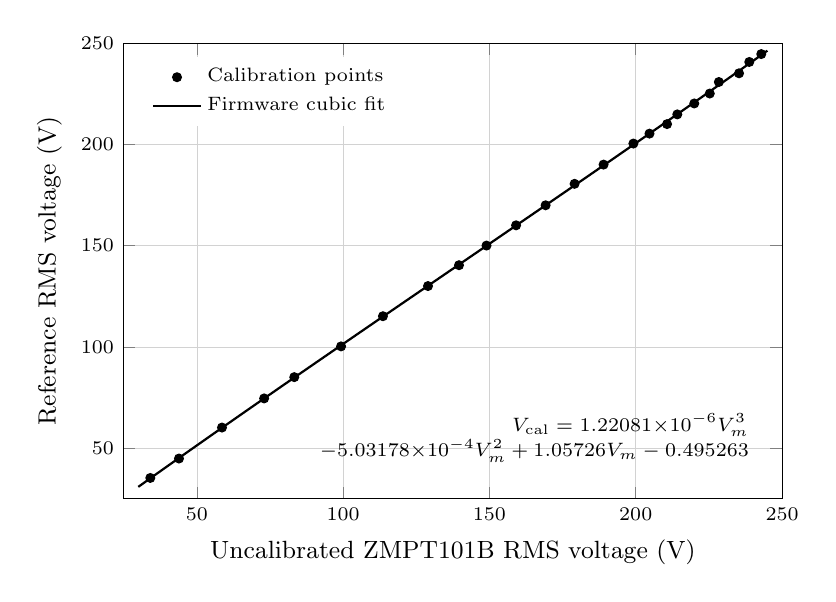
\begin{tikzpicture}
    \begin{axis}[
      width=0.82\textwidth,
      height=2.9in,
      xlabel={Uncalibrated ZMPT101B RMS voltage (V)},
      ylabel={Reference RMS voltage (V)},
      xmin=25,
      xmax=250,
      ymin=25,
      ymax=250,
      grid=major,
      major grid style={line width=0.2pt,draw=gray!35},
      tick label style={font=\scriptsize},
      label style={font=\small},
      legend style={font=\scriptsize,draw=none,at={(0.03,0.97)},anchor=north west},
      legend cell align={left}
    ]
      \addplot[only marks,mark=*,mark size=1.6pt,black] coordinates {
        (34.1,35.2) (43.9,44.79) (58.6,60.1) (73,74.5)
        (83.3,85) (99.3,100.2) (113.6,115.1) (129,130)
        (139.6,140.3) (149,150) (159.1,160) (169.2,169.9)
        (179.1,180.5) (189,190) (199.2,200.4) (204.7,205.3)
        (210.7,210) (214.2,214.8) (220,220.2) (225.3,225.1)
        (228.4,230.8) (235.3,235.1) (238.8,240.7) (242.9,244.6)
      };
      \addlegendentry{Calibration points}
      \addplot[black,thick,domain=30:245,samples=160]
        {1.22081e-6*x^3 - 5.03178e-4*x^2 + 1.05726*x - 0.495263};
      \addlegendentry{Firmware cubic fit}
      \node[anchor=south east,font=\scriptsize,align=right] at (axis cs:242,38)
        {$V_{\mathrm{cal}}=1.22081{\times}10^{-6}V_m^3$\\
         $-5.03178{\times}10^{-4}V_m^2+1.05726V_m-0.495263$};
    \end{axis}
  \end{tikzpicture}
  \caption{Cubic regression for voltage calibration.}
  \label{fig:ch3-voltage-regression}
\end{figure}

Figure~\ref{fig:ch3-voltage-regression} supports the cubic correction used by
the firmware. The implemented voltage calibration is
\begin{equation}
  V_{\mathrm{cal}} =
  1.22081\times10^{-6}V_m^3
  - 5.03178\times10^{-4}V_m^2
  + 1.05726V_m
  - 0.495263 .
  \label{eq:voltage-calibration}
\end{equation}
In (\ref{eq:voltage-calibration}), $V_m$ is the measured RMS voltage before
the cubic correction and $V_{\mathrm{cal}}$ is the calibrated RMS voltage used
for display and voltage protection. The polynomial correction is needed
because threshold decisions such as undervoltage, overvoltage, and
mains-present detection depend on the calibrated value.

\subsection{Current Calibration}
\label{sec:ch3-current-calibration}

The current calibration setup and load combinations are shown in
Figures~\ref{fig:ch3-current-cal-setup} and~\ref{fig:ch3-current-cal-loads}.

\begin{figure}[H]
  \centering
  
\includegraphics[width=0.90\textwidth]{ch3/figure_3.19.png}
  \caption{Data-collection setup for current calibration.}
  \label{fig:ch3-current-cal-setup}
\end{figure}

\begin{figure}[H]
  \centering
  
\includegraphics[width=0.90\textwidth]{ch3/figure_3.20.png}
  \caption{Load setups used for current calibration.}
  \label{fig:ch3-current-cal-loads}
\end{figure}

Figure~\ref{fig:ch3-current-cal-setup} shows the comparison between the
prototype current channel and a reference instrument.
Figure~\ref{fig:ch3-current-cal-loads} shows the different resistive and
appliance loads used to span the current range needed for overload and
arc-feature testing.

The fitted current regression is shown in
Figure~\ref{fig:ch3-current-regression}.
\begin{figure}[H]
  \centering
  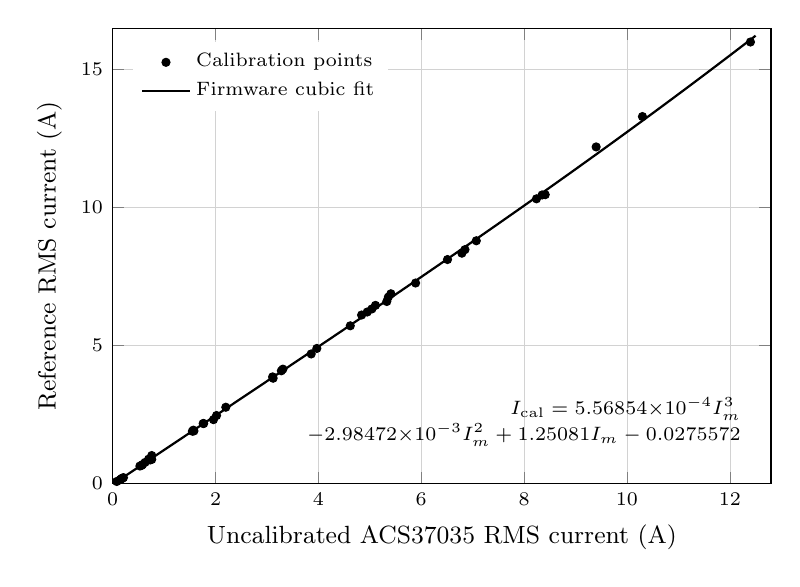
\begin{tikzpicture}
    \begin{axis}[
      width=0.82\textwidth,
      height=2.9in,
      xlabel={Uncalibrated ACS37035 RMS current (A)},
      ylabel={Reference RMS current (A)},
      xmin=0,
      xmax=12.8,
      ymin=0,
      ymax=16.5,
      grid=major,
      major grid style={line width=0.2pt,draw=gray!35},
      tick label style={font=\scriptsize},
      label style={font=\small},
      legend style={font=\scriptsize,draw=none,at={(0.03,0.97)},anchor=north west},
      legend cell align={left}
    ]
      \addplot[only marks,mark=*,mark size=1.45pt,black] coordinates {
        (0.08,0.08) (0.15,0.15) (0.17,0.18) (0.19,0.2)
        (0.21,0.22) (0.53,0.64) (0.56,0.66) (0.58,0.69)
        (0.63,0.77) (0.73,0.86) (0.76,0.88) (0.7,0.89)
        (0.76,1.02) (1.55,1.9) (1.58,1.91) (1.57,1.94)
        (1.76,2.18) (1.77,2.18) (1.96,2.32) (2.02,2.47)
        (2.2,2.77) (3.12,3.82) (3.11,3.87) (3.28,4.09)
        (3.31,4.15) (3.86,4.7) (3.97,4.9) (5.89,7.27)
        (4.62,5.72) (4.84,6.11) (4.95,6.22) (5.04,6.33)
        (5.11,6.46) (5.33,6.6) (5.36,6.76) (5.41,6.88)
        (6.51,8.12) (6.79,8.35) (6.85,8.48) (7.07,8.8)
        (8.24,10.32) (8.35,10.46) (8.41,10.47) (9.4,12.2)
        (10.3,13.3) (12.4,16)
      };
      \addlegendentry{Calibration points}
      \addplot[black,thick,domain=0:12.5,samples=160]
        {5.56854e-4*x^3 - 2.98472e-3*x^2 + 1.25081*x - 0.0275572};
      \addlegendentry{Firmware cubic fit}
      \node[anchor=south east,font=\scriptsize,align=right] at (axis cs:12.4,1.0)
        {$I_{\mathrm{cal}}=5.56854{\times}10^{-4}I_m^3$\\
         $-2.98472{\times}10^{-3}I_m^2+1.25081I_m-0.0275572$};
    \end{axis}
  \end{tikzpicture}
  \caption{Cubic regression for current calibration.}
  \label{fig:ch3-current-regression}
\end{figure}

The implemented current calibration is
\begin{equation}
  I_{\mathrm{cal}} =
  5.56854\times10^{-4}I_m^3
  - 2.98472\times10^{-3}I_m^2
  + 1.25081I_m
  - 0.0275572 .
  \label{eq:current-calibration}
\end{equation}
In (\ref{eq:current-calibration}), $I_m$ is the measured RMS current before
the cubic correction and $I_{\mathrm{cal}}$ is the calibrated RMS current used
by the overload logic, socket-temperature model, and waveform-feature
extractor. Negative fitted values are clamped to zero in firmware.

The device temperature measurement calibration setup is shown in
Figure~\ref{fig:ch3-ntc-cal-setup}.

\subsection{Device Temperature Measurement Calibration}
\label{sec:ch3-device-temperature-calibration}

\begin{figure}[H]
  \centering
  
\includegraphics[width=0.85\textwidth]{ch3/figure_3.22.jpg}
  \caption{Data-collection setup for device temperature measurement calibration.}
  \label{fig:ch3-ntc-cal-setup}
\end{figure}

Figure~\ref{fig:ch3-ntc-cal-setup} shows the external thermistor measurement
being compared with a reference temperature measurement. Thermistor placement
is important because an external sensor can lag or under-read the hottest
contact point inside a degraded socket [27], [29], [30]. The acquired
temperature-resistance calibration points are listed in
Table~\ref{tab:app-a-temperature-calibration}.

The firmware computes the NTC resistance from the voltage-divider output:
\begin{equation}
  R_{\mathrm{NTC}} =
  \frac{V_{\mathrm{NTC}}R_D}{V_{\mathrm{CC}} - V_{\mathrm{NTC}}}.
  \label{eq:ntc-resistance}
\end{equation}
In (\ref{eq:ntc-resistance}), $V_{\mathrm{NTC}}$ is the measured divider
voltage, $R_D=3.3\mathrm{k}\Omega$ is the fixed divider resistor, and
$V_{\mathrm{CC}}=3.3\mathrm{V}$ is the divider supply. The resistance is then
converted to temperature with the Beta equation:
\begin{equation}
  T_{\mathrm{NTC}} =
  \left[
  \frac{1}{T_0} +
  \frac{1}{\beta}\ln\left(\frac{R_{\mathrm{NTC}}}{R_0}\right)
  \right]^{-1}
  - 273.15 .
  \label{eq:ntc-beta}
\end{equation}
In (\ref{eq:ntc-beta}), $T_{\mathrm{NTC}}$ is in degrees Celsius, $T_0 =
298.15\mathrm{K}$, $R_0=10\mathrm{k}\Omega$, and $\beta=4050$. The
computed temperature is clamped from $-20\degreeC$ to $125\degreeC$ and
filtered with a 3s time constant in the temperature-sensing routine.

\section{Socket-Heating Temperature Models}
\label{sec:ch3-socket-heating-models}

The socket-heating computation uses two related models. The first is the
expected normal socket temperature, which estimates the socket temperature
expected under healthy contact behavior. The second is the estimated socket
temperature, which is the protection-facing compensated value intended to
respond to degraded-contact heating and external device temperature under-reading. This
separation is necessary because a raw external thermistor does not directly
measure the internal contact hotspot [30], [46], [47].

\subsection{Expected Normal Temperature Model}
\label{sec:ch3-expected-normal-temperature}

The firmware first decides whether the load is active:
\begin{equation}
  L =
  \begin{cases}
  1, & \text{if mains is present and } I_{\mathrm{rms}}\geq 0.35\mathrm{A},\\
  0, & \text{otherwise}.
  \end{cases}
  \label{eq:load-active}
\end{equation}
In (\ref{eq:load-active}), $L$ is the load-active flag and
$I_{\mathrm{rms}}$ is the calibrated RMS current. When $L=0$, the current
dependent thermal rise is forced toward zero.

The current-dependent shape term is
\begin{equation}
  s_I =
  \left[
  \mathrm{clamp}\left(\frac{I_{\mathrm{rms}}}{12.0},\,0,\,1.25\right)
  \right]^2 .
  \label{eq:thermal-current-shape}
\end{equation}
In (\ref{eq:thermal-current-shape}), $s_I$ is the normalized squared current
term. The 12.0A denominator and 1.25 clamp are firmware constants. The square
term reflects that heat generation associated with resistive loss rises with
current squared.

The ambient or baseline term is tracked from the device temperature measurement only when the
load is off or the current is below 0.18A:
\begin{equation}
  T_a[k] = T_a[k-1] + \alpha_a\left(T_{\mathrm{NTC}}[k] - T_a[k-1]\right),
  \qquad
  \alpha_a = \frac{\Delta t}{240\mathrm{s}} .
  \label{eq:thermal-ambient}
\end{equation}
In (\ref{eq:thermal-ambient}), $T_a$ is the inferred ambient or baseline
temperature, $\Delta t$ is the elapsed firmware update time, and
$T_{\mathrm{NTC}}$ is the measured thermistor temperature. The 240s time
constant prevents the baseline from following short-term load heating.

The target normal rise is
\begin{equation}
  \Delta T_{\mathrm{normal,target}} =
  \begin{cases}
  0.20 + 12.0s_I, & L=1,\\
  0, & L=0 .
  \end{cases}
  \label{eq:normal-target-rise}
\end{equation}
In (\ref{eq:normal-target-rise}), $0.20\degreeC$ is the normal base rise and
$12.0\degreeC$ is the normal current-rise gain. The fitted-gain source file
was not present in the codebase; the least-squares derivation should therefore
be checked against Appendix~\ref{app:c} or the original characterization
worksheet.

The firmware filters this target with separate heating and cooling time
constants:
\begin{equation}
  \Delta T_{\mathrm{normal}}[k]
  =
  \Delta T_{\mathrm{normal}}[k-1]
  +
  \alpha_n\left(
  \Delta T_{\mathrm{normal,target}}[k] -
  \Delta T_{\mathrm{normal}}[k-1]\right).
  \label{eq:normal-rise-filter}
\end{equation}
In (\ref{eq:normal-rise-filter}), $\alpha_n=\Delta t/900\mathrm{s}$ when the
target rise is increasing and $\alpha_n=\Delta t/1800\mathrm{s}$ when the
target rise is decreasing. These time constants represent the slower thermal
response of the socket compared with the electrical measurements.

The expected normal socket temperature is then
\begin{equation}
  T_{\mathrm{normal,exp}} =
  \mathrm{clamp}
  \left(T_a + \Delta T_{\mathrm{normal}},\, -20,\,125\right).
  \label{eq:expected-normal-socket}
\end{equation}
In (\ref{eq:expected-normal-socket}), $T_{\mathrm{normal,exp}}$ is the
baseline or normal thermal estimate. It represents what the socket temperature
should be under expected contact behavior for the measured current history.

\subsection{Estimated Socket Temperature Model}
\label{sec:ch3-estimated-socket-temperature-model}

The measured device temperature value is compensated directly:
\begin{equation}
  T_{\mathrm{comp}} =
  \mathrm{clamp}
  \left(T_{\mathrm{NTC}} + \Delta T_{\mathrm{meas}},\, -20,\,125\right),
  \qquad
  \Delta T_{\mathrm{meas}} =
  \begin{cases}
  0.30 + 1.20s_I, & L=1,\\
  0, & L=0 .
  \end{cases}
  \label{eq:measured-compensation}
\end{equation}
In (\ref{eq:measured-compensation}), $T_{\mathrm{comp}}$ is the compensated
thermistor-based estimate, $0.30\degreeC$ is the measured base delta, and
$1.20\degreeC$ is the measured current gain. These constants were verified
from the firmware configuration; their original least-squares fitting
worksheet must be verified manually if the derivation is required in the final
defense copy.

Finally, the protection-facing socket estimate is
\begin{equation}
  T_{\mathrm{socket,est}} =
  \mathrm{clamp}
  \left(
  \max\left(T_{\mathrm{comp}}, T_{\mathrm{normal,exp}}\right),
  -20,
  125
  \right).
  \label{eq:estimated-socket-temp}
\end{equation}
In (\ref{eq:estimated-socket-temp}), $T_{\mathrm{socket,est}}$ is the
estimated socket temperature used by the protection manager. The maximum
operation makes the estimator conservative: it does not allow the compensated
device temperature estimate to fall below the expected normal socket estimate when load
current indicates that some heating should be present.

The verified thermal constants are summarized in
Table~\ref{tab:ch3-thermal-constants}.
\begin{table}[H]
  \centering
  \caption{Socket-heating constants verified from firmware}
  \label{tab:ch3-thermal-constants}
  \begin{tabular}{p{0.40\textwidth}p{0.20\textwidth}p{0.30\textwidth}}
    \toprule
    \textbf{Constant} & \textbf{Value} & \textbf{Function} \\
    \midrule
    Load-on current threshold & 0.35A & Enables current-dependent heating model \\
    Ambient tracking current limit & 0.18A & Allows baseline tracking only at very low load \\
    Ambient time constant & 240s & Slow baseline update \\
    Normal reference current & 12.0A & Denominator for current-shape term \\
    Normal base rise & 0.20°C & Minimum expected rise when load is active \\
    Normal current gain & 12.0°C & Expected normal heating gain \\
    Current-ratio clamp & 1.25 & Limits current-shape term \\
    Heating time constant & 900s & Rise filter for normal estimate \\
    Cooling time constant & 1800s & Fall filter for normal estimate \\
    Measured base delta & 0.30°C & Direct thermistor compensation offset \\
    Measured current gain & 1.20°C & Direct thermistor compensation gain \\
    Estimated-temperature trip threshold & 40.0°C & Thermal relay trip threshold \\
    Thermal warning and clear thresholds & 39.0°C / 38.6°C & Warning hysteresis \\
    \bottomrule
  \end{tabular}
\end{table}

Table~\ref{tab:ch3-thermal-constants} distinguishes the thermal estimator from
the warning and trip thresholds. The estimator produces
$T_{\mathrm{socket,est}}$, while the protection manager decides warning and
relay action from that estimate.

\subsection{Least-Squares Gain and Regression Derivation}
\label{sec:ch3-thermal-least-squares}

The intended calibration path for the socket-heating constants is to compare
the device temperature measurement and reference terminal readings against ambient, then
fit the compensation terms from the characterization records. For a gain-only
rise model, the least-squares gain is
\begin{equation}
  k =
  \frac{\sum_i x_i y_i}{\sum_i x_i^2},
  \label{eq:thermal-gain-fit}
\end{equation}
where $x_i$ is the predictor rise above ambient, such as device temperature measurement
rise or current-shaped rise, and $y_i$ is the reference terminal rise above
ambient. When an offset is required, the corresponding linear model is
\begin{equation}
  \Delta T_{\mathrm{ref}} =
  a\Delta T_{\mathrm{device}} + b .
  \label{eq:thermal-linear-fit}
\end{equation}
In (\ref{eq:thermal-linear-fit}), $\Delta T_{\mathrm{ref}}$ is the infrared
thermometer or terminal-contact rise and $\Delta T_{\mathrm{device}}$ is the
external thermistor rise. If time lag is evident, the time series should be
aligned before fitting. The source worksheet used to choose the firmware
constants was not present in the repository, so the constants in
Table~\ref{tab:ch3-thermal-constants} are reported as verified firmware
constants and should be recomputed from Appendix~\ref{app:c} or the original
worksheet before final defense submission.

\subsection{Firmware Implementation of Constants}
\label{sec:ch3-thermal-firmware-constants}

As an example, consider a load-active frame at $I_{\mathrm{rms}}=9.04\mathrm{A}$.
The current-shape term in (\ref{eq:thermal-current-shape}) is
\[
  s_I=\left(\frac{9.04}{12.0}\right)^2=0.568 .
\]
The direct thermistor-compensation rise in
(\ref{eq:measured-compensation}) is therefore
$0.30+1.20(0.568)=0.982\degreeC$. If the device temperature measurement for that
frame is $38.2\degreeC$, the direct compensated estimate is
$T_{\mathrm{comp}}=39.18\degreeC$ before the final maximum operation. For the
same current, the normal target rise in (\ref{eq:normal-target-rise}) is
$0.20+12.0(0.568)=7.02\degreeC$. The final protection-facing estimate still
depends on the filtered normal-rise state and inferred ambient term, which is
why the method evaluates a thermal history rather than only a single
instantaneous current and device temperature reading.

\section{Waveform Feature Computation}
\label{sec:ch3-waveform-features}

The arc-detection firmware computes waveform features from current samples
rather than from RMS current alone. This is necessary because a series arc can
leave the load current below a conventional breaker trip level while still
introducing low-current gaps, restrike pulses, irregular zero-crossing
behavior, and mid/high-frequency energy [34], [35], [53], [54]. The firmware
uses a 512-sample frame at a 27kHz target sampling rate, with a 256-sample
hop. A Hann window is applied before the FFT to reduce spectral leakage, which
is standard practice in discrete Fourier analysis [70], [75].

The current RMS value used in the feature frame is computed as
\begin{equation}
  I_{\mathrm{rms}} =
  \sqrt{\frac{1}{N}\sum_{n=0}^{N-1} i[n]^2}.
  \label{eq:feature-rms}
\end{equation}
In (\ref{eq:feature-rms}), $i[n]$ is the calibrated current sample after the
firmware's current conversion path and $N$ is the number of samples in the
frame. RMS current represents the effective load current and is used both as a
protection variable and as a baseline reference for several arc features.

The firmware also computes current THD from the fundamental and harmonic tone
powers:
\begin{equation}
  \mathrm{THD}_I =
  100\sqrt{\frac{\sum_{h=2}^{10}P_h}{P_1}} .
  \label{eq:feature-thd}
\end{equation}
In (\ref{eq:feature-thd}), $P_1$ is the tracked fundamental tone power and
$P_h$ is the tone power of harmonic $h$. The firmware limits the harmonic sum
to available harmonics below Nyquist. THD is useful because arcing and
nonlinear loads can distort the current waveform, although THD alone is not
sufficient for reliable arc detection [35].

The mid/high-frequency spectral flux feature compares the normalized magnitude
spectrum of the present frame with the previous frame:
\begin{equation}
  F_{\mathrm{midhf}} =
  50\sum_{k=k_0}^{k_1}
  \left|
  \frac{M_k}{\sum_{r=k_0}^{k_1}M_r}
  -
  \frac{M_{k,\mathrm{prev}}}{\sum_{r=k_0}^{k_1}M_{r,\mathrm{prev}}}
  \right|.
  \label{eq:feature-spectral-flux}
\end{equation}
In (\ref{eq:feature-spectral-flux}), $M_k$ is the FFT magnitude in the 900Hz
to 9000Hz flux band after skipping bins around mains harmonics. The factor 50
comes from the firmware expression $0.5 \times 100$. This feature increases
when the mid/high-frequency spectrum changes abruptly from one frame to the
next, which is consistent with intermittent arc restrike behavior.

The high-frequency energy delta compares the high-frequency energy share with
its baseline:
\begin{equation}
  \Delta E_{\mathrm{HF}} =
  10\log_{10}
  \left(
  \frac{E_{\mathrm{HF}}/(E_{\mathrm{HF}}+E_{\mathrm{UM}})+\epsilon}
       {B_{\mathrm{HF}}+\epsilon}
  \right).
  \label{eq:feature-hf-delta}
\end{equation}
In (\ref{eq:feature-hf-delta}), $E_{\mathrm{HF}}$ is the 4500--9000Hz band
energy, $E_{\mathrm{UM}}$ is the 900--4500Hz upper-midband energy,
$B_{\mathrm{HF}}$ is the baseline high-frequency share, and $\epsilon$ is a
small numerical offset. This feature detects a rise in high-frequency content
relative to recent non-arcing operation.

The midband residual ratio is computed from FFT energy in the 220--3200Hz
midband after excluding harmonic bins:
\begin{equation}
  R_{\mathrm{mid}} =
  20\log_{10}
  \left(
  \frac{\sqrt{E_{\mathrm{mid,res}}}/N}
       {\max(B_I,\,0.10)}
  \right).
  \label{eq:feature-midband-ratio}
\end{equation}
In (\ref{eq:feature-midband-ratio}), $E_{\mathrm{mid,res}}$ is the residual
midband energy, $N$ is the frame length, and $B_I$ is the baseline RMS current.
The firmware uses a 0.10A floor to prevent division by a near-zero baseline.
This feature emphasizes non-harmonic disturbance relative to the normal current
level.

The low-current ratio measures the portion of the frame close to zero current:
\begin{equation}
  L_{\mathrm{ratio}} =
  \frac{100}{N}\sum_{n=0}^{N-1}
  \mathbf{1}
  \left(
  |i_c[n]| \leq
  \max(0.035,\,0.06\max(I_{\mathrm{rms}},0.10))
  \right).
  \label{eq:feature-low-current-ratio}
\end{equation}
In (\ref{eq:feature-low-current-ratio}), $i_c[n]$ is the cleaned current
sample and $\mathbf{1}(\cdot)$ is an indicator function. The 0.035A floor and
0.06 current fraction were verified from the firmware configuration. A high
low-current ratio can indicate current interruption or gap behavior during a
series arc.

The maximum low-current run is computed as
\begin{equation}
  t_{\mathrm{low,max}} =
  \frac{1000\,N_{\mathrm{run,max}}}{f_s}.
  \label{eq:feature-low-current-run}
\end{equation}
In (\ref{eq:feature-low-current-run}), $N_{\mathrm{run,max}}$ is the longest
consecutive run of samples satisfying the low-current condition in
(\ref{eq:feature-low-current-ratio}) and $f_s$ is the sampling rate in hertz.
The result is expressed in milliseconds and is one of the six deployed
base features in the final arc model.

The RMS-current baseline z-score is
\begin{equation}
  Z_I =
  \frac{|I_{\mathrm{rms}}-\mu_I|}{\sigma_I+10^{-6}} .
  \label{eq:feature-irms-zscore}
\end{equation}
In (\ref{eq:feature-irms-zscore}), $\mu_I$ and $\sigma_I$ are the adaptive
baseline mean and standard deviation maintained by the firmware. The baseline
is frozen when arc-like features or large current steps are detected, which
prevents the baseline from immediately absorbing a fault signature.

The feature groups used by the firmware are summarized in
Table~\ref{tab:ch3-feature-groups}.
\begin{table}[H]
  \centering
  \caption{Waveform features and physical interpretation}
  \label{tab:ch3-feature-groups}
  \begin{tabular}{p{0.26\textwidth}p{0.34\textwidth}p{0.30\textwidth}}
    \toprule
    Feature group & Computation basis & Physical meaning \\
    \midrule
    RMS and z-score & Frame RMS and adaptive baseline & Load magnitude and unusual current change \\
    Low-current gap features & Low-current ratio, zero dwell, maximum low-current run & Current interruption and restrike gap behavior \\
    Spectral features & FFT bands, spectral flux, high-frequency energy delta & Broadband and frame-to-frame disturbance \\
    Residual features & Cleaned waveform minus low-frequency baseline & Non-harmonic spikes and midband disturbance \\
    Shape features & Cycle NMSE, peak fluctuation, half-cycle asymmetry & Irregular cycle shape and asymmetry \\
    Pulse features & Residual pulse count per cycle & Short spikes consistent with arc restrike \\
    \bottomrule
  \end{tabular}
\end{table}

Table~\ref{tab:ch3-feature-groups} shows why the final classifier used a
combination of features. No single feature is expected to identify all arc
faults across appliance families; the classifier instead combines gap,
spectral, residual, and context information.

\section{Fault Detection and Protection Logic}
\label{sec:ch3-protection-logic}

The protection manager receives calibrated voltage, calibrated RMS current,
estimated socket temperature, and TinyML arc output. It then assigns warning
and trip states according to thresholds and persistence rules in the firmware.
The relay is opened only after a trip condition is accepted by the protection
logic; warnings alone do not disconnect the load.

\subsection{Voltage Supervision}
\label{sec:ch3-voltage-protection}

Voltage supervision uses calibrated RMS voltage and mains-present state. The
firmware defines the normal operating band as 200-250V. Instantaneous
undervoltage protection is set at 170V, delayed undervoltage is set below
200V for 7s, delayed overvoltage is set above 250V for 7s, and
instantaneous overvoltage is set at 260V. Recovery requires the voltage to
return to 212-250V and remain stable for 5min.

These thresholds are treated as design choices for supply-state supervision
rather than validated voltage-protection performance, since the experimental
validation focused on fire-inducing fault types. The implemented values are
summarized in \textit{Table~\ref{tab:ch3-voltage-thresholds}}.

\begin{table}[H]
  \centering
  \caption{Voltage-protection thresholds verified from firmware}
  \label{tab:ch3-voltage-thresholds}
  \begin{tabular}{@{}p{0.31\textwidth}p{0.17\textwidth}p{0.44\textwidth}@{}}
    \toprule
    \textbf{Condition} & \textbf{Firmware value} & \textbf{Interpretation} \\
    \midrule
    Normal lower limit & 200V & Lower edge of normal operation \\
    Normal upper limit & 250V & Upper edge of normal operation \\
    Instant undervoltage & 170V & Immediate severe undervoltage trip \\
    Delayed undervoltage & 200V for 7s & Persistent low-voltage trip \\
    Delayed overvoltage & 250V for 7s & Persistent high-voltage trip \\
    Instant overvoltage & 260V & Immediate severe overvoltage trip \\
    Recovery band & 212-250V for 5min & Stable voltage required before recovery \\
    \bottomrule
  \end{tabular}
\end{table}

\textit{Table~\ref{tab:ch3-voltage-thresholds}} shows that the voltage logic includes
both instantaneous and delayed decisions. This avoids treating every brief
voltage excursion as a latched trip while still allowing severe voltage
conditions to disconnect promptly.

\subsection{Overload Protection}
\label{sec:ch3-overload-protection}

The overload logic separates warning from relay trip. A warning begins when
current exceeds 10.0A after the warning delay and clears below 9.6A. A
sustained-overload trip requires the current average to remain above 14.5A
long enough for the overload score to reach the trip score.

The persistence score is represented as
\begin{equation}
  S_{\mathrm{OL}}[k] =
  \min\left(S_{\max}, S_{\mathrm{OL}}[k-1] + 1\right),
  \qquad I_{\mathrm{avg}}\geq 14.5\mathrm{A},
  \label{eq:overload-score-rise}
\end{equation}
and
\begin{equation}
  S_{\mathrm{OL}}[k] =
  \max\left(0, S_{\mathrm{OL}}[k-1] - 1\right),
  \qquad I_{\mathrm{avg}}\leq 14.1\mathrm{A}.
  \label{eq:overload-score-fall}
\end{equation}
In (\ref{eq:overload-score-rise}) and (\ref{eq:overload-score-fall}),
$S_{\mathrm{OL}}$ is the sustained-overload score, $I_{\mathrm{avg}}$ is the
firmware's 1s averaged current, and $S_{\max}=6$. The score is updated every
10s, and relay trip occurs at $S_{\mathrm{OL}}=6$. Therefore, a persistent
overload near or above 14.5A trips after about 60s, while shorter excursions
can produce warnings without disconnection. Persistence-based behavior is
consistent with the principle that overcurrent protection should distinguish
brief transients from sustained thermal stress [22].

\subsection{Socket-Heating Protection}
\label{sec:ch3-heating-protection}

Socket-heating protection uses the estimated socket temperature
$T_{\mathrm{socket,est}}$ from (\ref{eq:estimated-socket-temp}). The firmware
uses a warning threshold of $39.0\degreeC$, a warning-clear threshold of
$38.6\degreeC$, and a trip threshold of $40.0\degreeC$. The warning hysteresis
reduces rapid warning toggling near the threshold, while the trip threshold
creates a conservative response to possible contact heating.

The trip rule is
\begin{equation}
  H =
  \begin{cases}
  1, & T_{\mathrm{socket,est}}\geq 40.0\degreeC,\\
  0, & T_{\mathrm{socket,est}}<40.0\degreeC .
  \end{cases}
  \label{eq:heating-trip-rule}
\end{equation}
In (\ref{eq:heating-trip-rule}), $H$ is the heating-trip state. This trip
criterion is intentionally based on the compensated socket estimate rather
than the direct device temperature measurement because the external thermistor can under-read the
contact hotspot during degraded-contact heating [30], [46], [47].

\subsection{Series Arc-Fault Protection}
\label{sec:ch3-arc-protection}

The Random Forest arc model produces a frame-level arc class. The protection
manager does not trip from a single isolated model output. Instead, the
firmware uses a leaky counter:
\begin{equation}
  C_{\mathrm{arc}}[k] =
  \min\left(16, C_{\mathrm{arc}}[k-1] + 2\right),
  \qquad \hat{y}_{\mathrm{arc}}=1,
  \label{eq:arc-counter-rise}
\end{equation}
and
\begin{equation}
  C_{\mathrm{arc}}[k] =
  \max\left(0, C_{\mathrm{arc}}[k-1] - 6\right),
  \qquad \hat{y}_{\mathrm{arc}}=0 .
  \label{eq:arc-counter-fall}
\end{equation}
In (\ref{eq:arc-counter-rise}) and (\ref{eq:arc-counter-fall}),
$C_{\mathrm{arc}}$ is the arc persistence counter and
$\hat{y}_{\mathrm{arc}}$ is the TinyML model output. The relay trips when
$C_{\mathrm{arc}}\geq 8$. The counter therefore requires repeated arc-positive
frames and quickly decays when the classifier output returns to normal.

The firmware also includes a current-return verification path. If current
falls below 0.03A before the arc counter reaches the trip threshold, the
system waits up to 200ms to verify whether current returns before treating the
event as an arc trip. This guards against disconnecting on a simple load turn
off while still allowing fast response to arc-like interruption and restrike.

\subsection{Protection Priority and Latching}
\label{sec:ch3-priority-latching}

When multiple protection conditions are present, the firmware resolves the
reported fault according to protection priority. Socket heating is given the
highest priority because temperature is the most direct indicator of thermal
fire risk, followed by arc fault, sustained overload, and voltage-related
protection states. The relay-latching circuit is pulsed by the firmware after a
trip decision, and the fault state remains latched until the user clears it.
This prioritization does not change the underlying detection equations; it only
determines which fault reason is reported when conditions overlap.

The principal thresholds are summarized in \textit{Table~\ref{tab:ch3-protection-summary}}.
\begin{table}[H]
  \centering
  \caption{Principal protection thresholds verified from firmware}
  \label{tab:ch3-protection-summary}
  \begin{tabular}{p{0.26\textwidth}p{0.30\textwidth}p{0.34\textwidth}}
    \toprule
    \textbf{Protection function} & \textbf{Warning or model threshold} & \textbf{Relay-trip condition} \\
    \midrule
    Voltage supervision & Outside 200--250V band & Instant 170/260V or delayed 7s low/high voltage \\
    Overload & Warning above 10.0A; clear below 9.6A & 1s current average at or above 14.5A for about 60s \\
    Socket heating & Warning at 39.0°C; clear at 38.6°C & Estimated socket temperature at or above 40.0°C \\
    Series arc fault & RF probability threshold depends on context & Arc counter reaches 8 from repeated arc-positive frames \\
    \bottomrule
  \end{tabular}
\end{table}

\textit{Table~\ref{tab:ch3-protection-summary}} shows that the prototype uses a hybrid
method: deterministic thresholds for voltage, overload, and temperature, and
TinyML-supported classification for series arcs. The hybrid design is intended
to complement existing protection devices by observing socket-level thermal
and waveform behavior that may not be sufficient to trip a branch breaker.


\section{Test and Evaluation Procedures}
\label{sec:ch3-test-evaluation}

The evaluation followed the same order as the implementation: sensor
validation, overload testing, socket-heating characterization,
socket-heating protection validation, series arc-fault testing, and TinyML
model evaluation. Full calibration records are placed in
Appendix~\ref{app:a}; socket-heating characterization and protection data are
placed in Appendices~\ref{app:c} and~\ref{app:d}; arc-fault testing and data
collection logs are placed in Appendices~\ref{app:e} and~\ref{app:f}. The
letters, safety proposal, project schedule, and cost documentation are placed
in Appendices~\ref{app:g},~\ref{app:h}, and~\ref{app:i}.

\subsection{Sensor-Validation Metrics}
\label{sec:ch3-sensor-metrics}

Sensor validation compared prototype readings against reference instruments.
The mean absolute error was computed as
\begin{equation}
  \mathrm{MAE} =
  \frac{1}{n}\sum_{i=1}^{n}|y_i-\hat{y}_i|.
  \label{eq:metric-mae}
\end{equation}
The mean squared error was computed as
\begin{equation}
  \mathrm{MSE} =
  \frac{1}{n}\sum_{i=1}^{n}(y_i-\hat{y}_i)^2.
  \label{eq:metric-mse}
\end{equation}
The root mean squared error was computed as
\begin{equation}
  \mathrm{RMSE} =
  \sqrt{\frac{1}{n}\sum_{i=1}^{n}(y_i-\hat{y}_i)^2}.
  \label{eq:metric-rmse}
\end{equation}
The mean absolute percentage error was computed as
\begin{equation}
  \mathrm{MAPE} =
  \frac{100}{n}\sum_{i=1}^{n}
  \left|\frac{y_i-\hat{y}_i}{y_i}\right|.
  \label{eq:metric-mape}
\end{equation}
In (\ref{eq:metric-mae})--(\ref{eq:metric-mape}), $y_i$ is the reference
measurement, $\hat{y}_i$ is the prototype measurement, and $n$ is the number of
test points. MAE gives the average magnitude of error, MSE and RMSE penalize
larger errors more strongly, and MAPE expresses the error relative to the
reference value [72].

\subsection{Overload Test Procedure}
\label{sec:ch3-overload-test-procedure}

Overload testing used high-power load combinations to determine whether the
prototype warned above the warning threshold and tripped only when the
sustained-overload condition persisted. The block diagram of the overload test
is shown in Figure~\ref{fig:ch3-overload-block}.
\begin{figure}[H]
  \centering
  \resizebox{0.96\textwidth}{!}{%
  \begin{tikzpicture}[node distance=0.34in and 0.36in]
    \node[thesis process,text width=1.35in] (supply) {230V AC supply\\with breaker access};
    \node[thesis process,text width=1.35in,right=of supply] (plug) {TinyML Smart Plug\\under test};
    \node[thesis process,text width=1.35in,right=of plug] (load) {High-power\\load bank};
    \node[thesis process,text width=1.55in,below=of plug] (log) {PWA logs\\current, warning, relay, latency};
    \draw[thesis arrow] (supply) -- (plug);
    \draw[thesis arrow] (plug) -- (load);
    \draw[thesis arrow] (plug) -- (log);
  \end{tikzpicture}%
  }
  \caption{Testing setup block diagram for overload evaluation.}
  \label{fig:ch3-overload-block}
\end{figure}

Figure~\ref{fig:ch3-overload-block} shows the prototype placed between the
supply and load bank so that it could measure current and disconnect the load
through its relay. This matches the current path used in normal operation.

The actual overload test setup is shown in Figure~\ref{fig:ch3-overload-actual}.
\begin{figure}[H]
  \centering
  
\includegraphics[width=0.88\textwidth]{ch3/figure_3.31.png}
  \caption{Actual test setup for overload evaluation.}
  \label{fig:ch3-overload-actual}
\end{figure}

Figure~\ref{fig:ch3-overload-actual} documents the physical load arrangement
used to create warning and sustained-overload conditions. During each trial,
mean voltage, mean current, peak current, warning state, relay state, and trip
latency were recorded.

\subsection{Socket-Heating Test Procedure}
\label{sec:ch3-heating-test-procedure}

Socket-heating tests compared normal and intentionally degraded socket
contacts under similar load levels. The objective was to determine whether
degraded contacts produced faster and higher temperature rise, and whether the
external device temperature measurement and compensated estimator could provide useful warning before
dangerous contact heating progressed.

Figure~\ref{fig:ch3-heating-block} shows the socket-heating test block
diagram.
\begin{figure}[H]
  \centering
  \resizebox{0.96\textwidth}{!}{%
  \begin{tikzpicture}[node distance=0.34in and 0.34in]
    \node[thesis process,text width=1.35in] (supply) {230V AC supply\\with breaker access};
    \node[thesis process,text width=1.35in,right=of supply] (plug) {Prototype\\thermistor channel};
    \node[thesis process,text width=1.35in,right=of plug] (socket) {Normal or degraded\\socket contact};
    \node[thesis process,text width=1.35in,right=of socket] (load) {Matched\\load case};
    \node[thesis process,text width=1.55in,below=of socket] (reference) {Infrared thermometer\\terminal/contact reading};
    \node[thesis process,text width=1.55in,below=of plug] (log) {Logs: device temperature measurement, estimate, terminal, relay};
    \draw[thesis arrow] (supply) -- (plug);
    \draw[thesis arrow] (plug) -- (socket);
    \draw[thesis arrow] (socket) -- (load);
    \draw[thesis arrow] (reference) -- (log);
    \draw[thesis arrow] (plug) -- (log);
  \end{tikzpicture}%
  }
  \caption{Testing setup block diagram for socket-heating evaluation.}
  \label{fig:ch3-heating-block}
\end{figure}

Figure~\ref{fig:ch3-heating-block} shows that both the prototype Device
Measurement and a reference socket or terminal temperature measurement were
observed during testing. This made it possible to distinguish device temperature measurement,
estimated socket temperature, and reference terminal temperature in the
results.

The degraded socket contacts are shown in Figure~\ref{fig:ch3-corroded-contacts}.
\begin{figure}[H]
  \centering
  
\includegraphics[width=0.80\textwidth]{ch3/figure_3.33.png}
  \caption{Corroded socket contacts used for degraded-contact testing.}
  \label{fig:ch3-corroded-contacts}
\end{figure}

Figure~\ref{fig:ch3-corroded-contacts} documents the degraded-contact
condition used to accelerate contact heating. The degraded socket was compared
against a normal socket under matched load combinations.

The actual socket-heating test setup is shown in
Figure~\ref{fig:ch3-heating-actual}.
\begin{figure}[H]
  \centering
  
\includegraphics[width=0.88\textwidth]{ch3/figure_3.34.png}
  \caption{Actual test setup for socket-heating evaluation.}
  \label{fig:ch3-heating-actual}
\end{figure}

Figure~\ref{fig:ch3-heating-actual} shows the bench configuration used to
record time, current, device temperature measurement, estimated socket temperature,
reference terminal temperature, and relay behavior. The characterization data
in Appendix~\ref{app:c} were used to support the thermal model, while the
protection validation data in Appendix~\ref{app:d} were used to evaluate
relay response.

\subsection{Series Arc-Fault Test Procedure}
\label{sec:ch3-arc-test-procedure}

Series arc-fault testing used a controlled arc platform and appliance loads.
The goal was to create repeatable waveform disturbances while recording
current features, model outputs, relay behavior, and event labels. The
assistance letter and safety proposal for this testing activity are included
in Appendix~\ref{app:g}. The arc platform is shown in
Figure~\ref{fig:ch3-arc-platform}.
\begin{figure}[H]
  \centering
  
\includegraphics[width=0.92\textwidth]{ch3/figure_3.35.png}
  \caption{Series arc-fault test platform.}
  \figsource{Qi et al., 2025 [48]}
  \label{fig:ch3-arc-platform}
\end{figure}

Figure~\ref{fig:ch3-arc-platform} shows the principle of the series arc test:
the current path is interrupted by an adjustable contact gap, allowing a
controlled arc disturbance to appear in series with the load. The adapted
source describes a 220V/50Hz platform using a fixed electrode and a moving
electrode controlled by a stepper motor [48]. The prototype testing used the
same series-interruption principle as a guide, while the actual bench setup
used in this study is documented in Figure~\ref{fig:ch3-arc-actual}.

The block diagram of the series arc-fault test is shown in
Figure~\ref{fig:ch3-arc-block}.
\begin{figure}[H]
  \centering
  \resizebox{0.96\textwidth}{!}{%
  \begin{tikzpicture}[node distance=0.34in and 0.34in]
    \node[thesis process,text width=1.25in] (supply) {230V AC supply\\with breaker access};
    \node[thesis process,text width=1.28in,right=of supply] (arc) {Series arc\\generator};
    \node[thesis process,text width=1.28in,right=of arc] (plug) {TinyML Smart Plug\\waveform logging};
    \node[thesis process,text width=1.28in,right=of plug] (load) {Appliance\\load};
    \node[thesis process,text width=1.55in,below=of plug] (label) {PWA/Python logs\\features, labels, relay};
    \draw[thesis arrow] (supply) -- (arc);
    \draw[thesis arrow] (arc) -- (plug);
    \draw[thesis arrow] (plug) -- (load);
    \draw[thesis arrow] (plug) -- (label);
  \end{tikzpicture}%
  }
  \caption{Testing setup block diagram for series arc-fault evaluation.}
  \label{fig:ch3-arc-block}
\end{figure}

Figure~\ref{fig:ch3-arc-block} shows the smart plug measuring the load current
while the arc generator is placed in series with the appliance. This setup is
consistent with the feature definitions in Section~\ref{sec:ch3-waveform-features},
which depend on current waveform disturbance.

The actual series arc-fault test setup is shown in
Figure~\ref{fig:ch3-arc-actual}.
\begin{figure}[H]
  \centering
  
\includegraphics[width=0.90\textwidth]{ch3/figure_3.37.png}
  \caption{Actual test setup for series arc-fault evaluation.}
  \label{fig:ch3-arc-actual}
\end{figure}

Figure~\ref{fig:ch3-arc-actual} documents the laboratory arrangement used to
collect arc and normal trials. Complete arc-fault test records are referenced
in Appendices~\ref{app:e} and~\ref{app:f}.

\subsection{Classification Metrics}
\label{sec:ch3-classification-metrics}

For arc-fault evaluation, the positive class was the arc-fault condition and
the negative class was normal operation. Accuracy, precision, recall, and
F1-score were computed from true positives (TP), false positives (FP), true
negatives (TN), and false negatives (FN):
\begin{equation}
  \mathrm{Accuracy} =
  \frac{\mathrm{TP}+\mathrm{TN}}
       {\mathrm{TP}+\mathrm{TN}+\mathrm{FP}+\mathrm{FN}},
  \label{eq:metric-accuracy}
\end{equation}
\begin{equation}
  \mathrm{Precision} =
  \frac{\mathrm{TP}}{\mathrm{TP}+\mathrm{FP}},
  \label{eq:metric-precision}
\end{equation}
\begin{equation}
  \mathrm{Recall} =
  \frac{\mathrm{TP}}{\mathrm{TP}+\mathrm{FN}},
  \label{eq:metric-recall}
\end{equation}
and
\begin{equation}
  F_1 =
  2\frac{\mathrm{Precision}\times\mathrm{Recall}}
        {\mathrm{Precision}+\mathrm{Recall}}.
  \label{eq:metric-f1}
\end{equation}
In (\ref{eq:metric-accuracy})--(\ref{eq:metric-f1}), precision measures how
many trip decisions were actually arc faults, recall measures how many arc
faults were detected, and F1-score summarizes the balance between false trips
and missed faults. These metrics are commonly used for supervised
classification and confusion-matrix evaluation [74].

